\documentclass[aspectratio=169]{beamer}
\beamertemplatenavigationsymbolsempty
\usepackage[utf8]{inputenc}
\usepackage[T1]{fontenc}
\usepackage{lmodern,bm,amsmath,amssymb,booktabs,tikz,pgfplots,graphicx}
\usepackage{tabularx,array,xcolor,colortbl,pifont,makecell,adjustbox}
\usetikzlibrary{positioning,arrows.meta,shapes.geometric,calc}
\pgfplotsset{compat=1.18}
% Design adapted from supplied main (16).tex; prior subject content excluded.
\newcommand{\good}[1]{\textcolor{green!50!black}{\textbf{#1}}}
\newcommand{\bad}[1]{\textcolor{red!70!black}{\textbf{#1}}}
\newcommand{\code}[1]{\texttt{\detokenize{#1}}}
\newcommand{\reportsource}[1]{{\vskip 0.4em\tiny\textcolor{gray!80!black}{\textbf{Source:} #1}\par}}
\newcommand{\scope}[1]{{\small\textit{#1}}\par\vspace{0.4em}}
\newcolumntype{Y}{>{\raggedright\arraybackslash}X}
\newcolumntype{P}[1]{>{\raggedright\arraybackslash}p{#1}}
\usetheme{Madrid}
\usecolortheme{beaver}
\setbeamertemplate{caption}[numbered]
\setlength{\tabcolsep}{4pt}
\renewcommand{\arraystretch}{1.12}
\pdfstringdefDisableCommands{\def\translate#1{#1}}
\tikzset{
 stage/.style={draw=gray!65,rounded corners=2pt,fill=gray!7,align=center,inner sep=5pt,minimum height=0.85cm},
 phys/.style={stage,fill=blue!7,draw=blue!45!black},
 outc/.style={stage,fill=green!8,draw=green!40!black},
 arr/.style={-{Stealth[length=1.8mm]},thick,gray!70!black},
 lab/.style={font=\tiny\itshape,fill=white,inner sep=1pt}}
\pgfplotsset{deckaxis/.style={axis lines*=left,tick label style={font=\footnotesize},
 label style={font=\footnotesize},title style={font=\small},grid style={gray!20},major tick length=2pt,scaled ticks=false}}
\title[NYgrid 2025]{Weekly Report}
\subtitle{Downstate Grid Refinement and 2025 Operating Inputs}
\author{Yifei Xu}
\institute{New York University}
\date{October 15, 2026}
\begin{document}
\maketitle

\begin{frame}{The 2019 Reference and the Current Model}
\scope{Liu et al., IEEE TPWRS 2023; 2019 is the example operating-data year}
\begin{center}
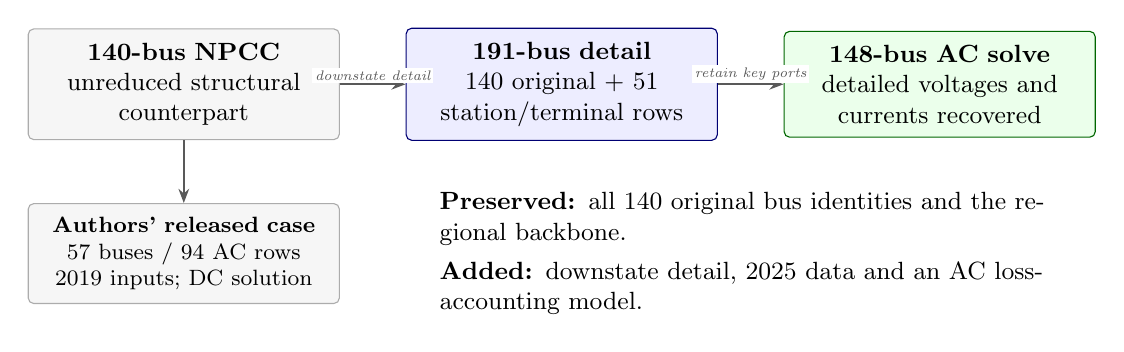
\begin{tikzpicture}[font=\small]
 \node[stage,text width=3.6cm] (base) at (0,0) {\textbf{140-bus NPCC}\\unreduced structural\\counterpart};
 \node[phys,text width=3.6cm] (detail) at (4.8,0) {\textbf{191-bus detail}\\140 original + 51\\station/terminal rows};
 \node[outc,text width=3.6cm] (ac) at (9.6,0) {\textbf{148-bus AC solve}\\detailed voltages and\\currents recovered};
 \draw[arr] (base)--node[lab,above]{downstate detail}(detail);
 \draw[arr] (detail)--node[lab,above]{retain key ports}(ac);
 \node[stage,text width=3.6cm,font=\footnotesize] (paper) at (0,-2.15) {\textbf{Authors' released case}\\57 buses / 94 AC rows\\2019 inputs; DC solution};
 \draw[arr] (base)--(paper);
 \node[align=left,text width=7.9cm,font=\small] at (7.2,-2.15) {\textbf{Preserved:} all 140 original bus identities and the regional backbone.\\[3pt]\textbf{Added:} downstate detail, 2025 data and an AC loss-accounting model.};
\end{tikzpicture}
\end{center}
\small The current expanded network has \textbf{266/267 buses}, including numerical line-section points---not 267 substations.
\reportsource{[1] Author-release audit; [2] downstate/slim construction; [4] current model inventory.}
\end{frame}

\begin{frame}{Downstate Network Modifications}
\centering
% Source-derived connectivity. Generated by build_downstate_figure.py.%
% Display positions are schematic. CSVs preserve every represented bus and circuit key.%
\begingroup%
\definecolor{dsAdded}{RGB}{140,24,48}%
\definecolor{dsOld}{RGB}{113,118,122}%
\begin{tikzpicture}[x=1cm,y=1cm, every node/.style={font=\fontsize{7.1}{8}\selectfont},%
 dsOriginal/.style={draw=dsOld,line width=.66pt},%
 dsAddedLine/.style={draw=dsAdded,line width=.55pt,opacity=.75},%
 dsLabel/.style={fill=white,inner sep=.7pt,text=black,align=left}]%
\path[use as bounding box] (0,0) rectangle (14.4,5.4);%
\node[anchor=west,font=\small\bfseries] at (.10,5.19) {2019 structural counterpart};%
\node[anchor=west,font=\small\bfseries] at (7.37,5.19) {Current downstate detail};%
\node[anchor=west,text=dsOld,font=\fontsize{8}{9}\selectfont] at (.10,4.88) {Paper-derived NPCC parent; G--K excerpt};%
\node[anchor=west,text=dsAdded,font=\fontsize{8}{9}\selectfont] at (7.37,4.88) {Station detail + dated projects};%
\draw[gray!25,line width=.4pt] (7.16,.54)--(7.16,5.35);%
% PARENT:32%
\draw[dsOriginal] (2.420,4.150) -- (6.420,4.150);%
% PARENT:87%
\draw[dsOriginal] (3.370,3.325) -- (2.420,4.150);%
% PARENT:88%
\draw[dsOriginal] (1.720,3.385) -- (3.370,3.325);%
% PARENT:89%
\draw[dsOriginal] (2.020,2.598) -- (3.370,3.325);%
% PARENT:91%
\draw[dsOriginal] (1.720,3.385) -- (0.670,3.460);%
% PARENT:92%
\draw[dsOriginal] (2.020,2.598) -- (6.420,2.590);%
% PARENT:93%
\draw[dsOriginal] (2.020,2.598) -- (5.770,3.062);%
% PARENT:94%
\draw[dsOriginal] (2.020,2.598) -- (0.620,1.000);%
% PARENT:95%
\draw[dsOriginal] (3.920,2.005) -- (2.020,2.598);%
\filldraw[draw=dsOld,fill=dsOld,line width=.55pt] (2.420,4.150) circle[radius=1.8pt];%
\filldraw[draw=dsOld,fill=dsOld,line width=.55pt] (0.670,3.460) circle[radius=1.8pt];%
\filldraw[draw=dsOld,fill=dsOld,line width=.55pt] (1.720,3.385) circle[radius=1.8pt];%
\filldraw[draw=dsOld,fill=dsOld,line width=.55pt] (3.370,3.325) circle[radius=1.8pt];%
\filldraw[draw=dsOld,fill=dsOld,line width=.55pt] (2.020,2.598) circle[radius=1.8pt];%
\filldraw[draw=dsOld,fill=dsOld,line width=.55pt] (6.420,2.590) circle[radius=1.8pt];%
\filldraw[draw=dsOld,fill=dsOld,line width=.55pt] (5.770,3.062) circle[radius=1.8pt];%
\filldraw[draw=dsOld,fill=dsOld,line width=.55pt] (0.620,1.000) circle[radius=1.8pt];%
\filldraw[draw=dsOld,fill=dsOld,line width=.55pt] (3.920,2.005) circle[radius=1.8pt];%
\filldraw[draw=dsOld,fill=dsOld,line width=.55pt] (6.420,4.150) circle[radius=1.8pt];%
% PERFORM:210, PERFORM:211%
\draw[dsAddedLine] (10.640,1.750) -- (8.290,1.780);%
% PERFORM:212, PERFORM:213%
\draw[dsAddedLine] (8.290,1.780) -- (8.770,2.237);%
% PERFORM:1107, PERFORM:1108, PERFORM:1109, PERFORM:1110%
\draw[dsAddedLine] (10.640,2.853) -- (10.190,3.107);%
% PERFORM:1111, PERFORM:1112, PERFORM:1113%
\draw[dsAddedLine] (10.640,3.325) -- (10.190,3.107);%
% PERFORM:1114%
\draw[dsAddedLine] (8.990,3.385) -- (10.190,3.107);%
% PERFORM:1159%
\draw[dsAddedLine] (10.090,2.598) -- (11.940,3.085);%
% PERFORM:1162%
\draw[dsAddedLine] (12.290,1.907) -- (12.840,1.765);%
% PERFORM:1164%
\draw[dsAddedLine] (11.870,2.215) -- (12.290,1.907);%
% PERFORM:1172, PERFORM:1173%
\draw[dsAddedLine] (12.840,1.765) -- (13.340,1.562);%
% PERFORM:1174, PERFORM:1175%
\draw[dsAddedLine] (12.840,2.590) -- (12.840,1.765);%
% PERFORM:1212, PERFORM:1213%
\draw[dsAddedLine] (13.340,1.225) -- (13.340,1.562);%
% PERFORM:1214, PERFORM:1215%
\draw[dsAddedLine] (12.840,2.590) -- (10.640,2.853);%
% PERFORM:1226, PERFORM:1227, PERFORM:1228, PERFORM:1229%
\draw[dsAddedLine] (10.090,2.598) -- (10.640,2.853);%
% PERFORM:1236, PERFORM:1237%
\draw[dsAddedLine] (10.640,2.853) -- (8.770,2.237);%
% PERFORM:1241, PERFORM:1242, PERFORM:1243%
\draw[dsAddedLine] (10.590,2.237) -- (10.190,2.365);%
% PERFORM:1245%
\draw[dsAddedLine] (10.640,1.750) -- (10.590,2.237);%
% PERFORM:1248, PERFORM:1249, PERFORM:1250%
\draw[dsAddedLine] (10.640,2.853) -- (11.140,2.485);%
% PERFORM:1257, PERFORM:1258%
\draw[dsAddedLine] (10.640,1.750) -- (10.990,1.465);%
% PERFORM:1260%
\draw[dsAddedLine] (11.870,2.215) -- (11.140,2.485);%
% PERFORM:1262, PERFORM:1263, PERFORM:1264%
\draw[dsAddedLine] (10.090,2.598) -- (10.190,2.365);%
% PERFORM:1265, PERFORM:1266, PERFORM:1267%
\draw[dsAddedLine] (11.410,1.585) -- (11.740,1.285);%
% PERFORM:1269, PERFORM:1270, PERFORM:1271, PERFORM:1272%
\draw[dsAddedLine] (10.640,1.750) -- (11.410,1.585);%
% PERFORM:1320, PERFORM:1321%
\draw[dsAddedLine] (12.490,0.925) -- (12.090,1.060);%
% PERFORM:1322, PERFORM:1323%
\draw[dsAddedLine] (12.490,0.925) -- (12.890,1.075);%
% PERFORM:1336, PERFORM:1337%
\draw[dsAddedLine] (11.740,1.285) -- (12.090,1.060);%
% PERFORM:1389, PERFORM:1390%
\draw[dsAddedLine] (10.240,3.925) -- (9.690,4.150);%
% PERFORM:1391, PERFORM:1392%
\draw[dsAddedLine] (9.690,4.150) -- (10.640,3.662);%
% PERFORM:1576%
\draw[dsAddedLine] (8.990,3.385) -- (8.440,3.700);%
% PERFORM:1577%
\draw[dsAddedLine] (8.440,3.700) -- (7.940,3.460);%
% PERFORM:1689, PERFORM:1690%
\draw[dsAddedLine] (10.240,3.925) -- (10.640,3.662);%
% PERFORM:1731, PERFORM:1732, PERFORM:1733%
\draw[dsAddedLine] (8.990,3.385) -- (10.640,3.325);%
% PERFORM:1734, PERFORM:1735%
\draw[dsAddedLine] (10.640,3.325) -- (10.640,3.662);%
% PERFORM:1738%
\draw[dsAddedLine] (8.990,3.385) -- (7.940,3.460);%
% PERFORM:1843, PERFORM:1844%
\draw[dsAddedLine] (12.890,1.075) -- (13.340,1.225);%
% PERFORM:1984, PERFORM:1985%
\draw[dsAddedLine] (8.870,1.292) -- (9.390,1.000);%
% PERFORM:1988, PERFORM:1989%
\draw[dsAddedLine] (8.870,1.292) -- (9.770,1.570);%
% PERFORM:1994%
\draw[dsAddedLine] (8.870,1.292) -- (8.210,1.413);%
% PERFORM:1997, PERFORM:1998, PERFORM:1999%
\draw[dsAddedLine] (9.770,1.570) -- (10.020,1.292);%
% PERFORM:2000%
\draw[dsAddedLine] (8.210,1.413) -- (8.770,2.237);%
% ATTACH:CEUG_DUNWOODIE%
\draw[dsAddedLine] (9.290,2.598) -- (10.090,2.598);%
% ATTACH:RAVA3_EGC%
\draw[dsAddedLine] (12.840,2.590) -- (13.690,2.590);%
% ATTACH:NORTHPORT_SHORERD%
\draw[dsAddedLine] (13.040,3.062) -- (11.940,3.085);%
% ATTACH:GOETHALS_GOWANUS%
\draw[dsAddedLine] (7.890,1.000) -- (9.390,1.000);%
% ATTACH:AK3_ASTORIA138%
\draw[dsAddedLine] (11.190,2.005) -- (10.640,1.750);%
% CV:BOUNDARY_SOUTHINGTON_LM%
\draw[dsAddedLine] (13.690,3.715) -- (13.690,4.150);%
% CV:PV_CV_F83_PROXY, CV:PV_CV_F84%
\draw[dsAddedLine] (11.690,4.150) -- (9.690,4.150);%
% DOVER:CV_DOVER_Y17%
\draw[dsAddedLine] (11.690,4.150) -- (12.690,4.113);%
% RECEIVING:GREENWOOD_CORONA%
\draw[dsAddedLine] (11.410,1.585) -- (10.340,0.902);%
% RECEIVING:FOXHILLS_GREENWOOD%
\draw[dsAddedLine] (8.790,0.790) -- (10.340,0.902);%
% ASSET:ANNEX_E13_Q35_PROXY%
\draw[dsAddedLine] (9.290,1.780) -- (8.290,1.780);%
% ASSET:FRESHKILLS138_FOXHILLS%
\draw[dsAddedLine] (8.310,0.640) -- (8.790,0.790);%
% ASSET:FRESHKILLS345_GOETHALS%
\draw[dsAddedLine] (7.740,0.640) -- (7.890,1.000);%
% RCC:PAR:GOWANUS%
\draw[dsAddedLine] (9.390,1.000) -- (9.790,1.000);%
% RCC:PAR:GOETHALS%
\draw[dsAddedLine] (7.890,1.000) -- (8.340,0.902);%
% RCC:PAR:RAINEY%
\draw[dsAddedLine] (9.770,1.570) -- (10.370,1.540);%
% RCC:CABLE:QUEENS%
\draw[dsAddedLine] (11.410,1.585) -- (10.370,1.540);%
% RCC:CABLE:BROOKLYN%
\draw[dsAddedLine] (10.340,0.902) -- (9.790,1.000);%
% RCC:CABLE:STATEN%
\draw[dsAddedLine] (8.790,0.790) -- (8.340,0.902);%
% DOVER:RESOLVED_398%
\draw[dsAddedLine] (12.690,4.113) -- (13.690,3.715);%
\filldraw[draw=dsOld,fill=dsOld,line width=.55pt] (9.690,4.150) circle[radius=1.8pt];%
\filldraw[draw=dsOld,fill=dsOld,line width=.55pt] (7.940,3.460) circle[radius=1.8pt];%
\filldraw[draw=dsOld,fill=dsOld,line width=.55pt] (8.990,3.385) circle[radius=1.8pt];%
\filldraw[draw=dsOld,fill=dsOld,line width=.55pt] (10.640,3.325) circle[radius=1.8pt];%
\filldraw[draw=dsOld,fill=dsOld,line width=.55pt] (9.290,2.598) circle[radius=1.8pt];%
\filldraw[draw=dsOld,fill=dsOld,line width=.55pt] (13.690,2.590) circle[radius=1.8pt];%
\filldraw[draw=dsOld,fill=dsOld,line width=.55pt] (13.040,3.062) circle[radius=1.8pt];%
\filldraw[draw=dsOld,fill=dsOld,line width=.55pt] (7.890,1.000) circle[radius=1.8pt];%
\filldraw[draw=dsOld,fill=dsOld,line width=.55pt] (11.190,2.005) circle[radius=1.8pt];%
\filldraw[draw=dsAdded,fill=dsAdded,line width=.55pt] (10.240,3.925) circle[radius=1.8pt];%
\filldraw[draw=dsAdded,fill=dsAdded,line width=.55pt] (10.640,3.662) circle[radius=1.8pt];%
\filldraw[draw=dsAdded,fill=dsAdded,line width=.55pt] (8.440,3.700) circle[radius=1.8pt];%
\filldraw[draw=dsAdded,fill=dsAdded,line width=.55pt] (11.690,4.150) circle[radius=1.8pt];%
\filldraw[draw=dsAdded,fill=white,line width=.55pt] (12.690,4.113) circle[radius=1.25pt];%
\filldraw[draw=dsAdded,fill=white,line width=.55pt] (13.690,3.715) circle[radius=1.25pt];%
\filldraw[draw=dsOld,fill=dsOld,line width=.55pt] (13.690,4.150) circle[radius=1.8pt];%
\filldraw[draw=dsAdded,fill=white,line width=.55pt] (10.190,3.107) circle[radius=1.25pt];%
\filldraw[draw=dsAdded,fill=white,line width=.55pt] (10.640,2.853) circle[radius=1.25pt];%
\filldraw[draw=dsAdded,fill=dsAdded,line width=.55pt] (10.090,2.598) circle[radius=1.8pt];%
\filldraw[draw=dsAdded,fill=white,line width=.55pt] (11.940,3.085) circle[radius=1.25pt];%
\filldraw[draw=dsAdded,fill=dsAdded,line width=.55pt] (12.840,2.590) circle[radius=1.8pt];%
\filldraw[draw=dsAdded,fill=white,line width=.55pt] (11.870,2.215) circle[radius=1.25pt];%
\filldraw[draw=dsAdded,fill=white,line width=.55pt] (12.290,1.907) circle[radius=1.25pt];%
\filldraw[draw=dsAdded,fill=white,line width=.55pt] (12.840,1.765) circle[radius=1.25pt];%
\filldraw[draw=dsAdded,fill=white,line width=.55pt] (13.340,1.562) circle[radius=1.25pt];%
\filldraw[draw=dsAdded,fill=white,line width=.55pt] (13.340,1.225) circle[radius=1.25pt];%
\filldraw[draw=dsAdded,fill=white,line width=.55pt] (12.890,1.075) circle[radius=1.25pt];%
\filldraw[draw=dsAdded,fill=white,line width=.55pt] (12.490,0.925) circle[radius=1.25pt];%
\filldraw[draw=dsAdded,fill=white,line width=.55pt] (12.090,1.060) circle[radius=1.25pt];%
\filldraw[draw=dsAdded,fill=white,line width=.55pt] (10.190,2.365) circle[radius=1.25pt];%
\filldraw[draw=dsAdded,fill=white,line width=.55pt] (10.590,2.237) circle[radius=1.25pt];%
\filldraw[draw=dsAdded,fill=white,line width=.55pt] (11.140,2.485) circle[radius=1.25pt];%
\filldraw[draw=dsAdded,fill=white,line width=.55pt] (10.640,1.750) circle[radius=1.25pt];%
\filldraw[draw=dsAdded,fill=white,line width=.55pt] (10.990,1.465) circle[radius=1.25pt];%
\filldraw[draw=dsAdded,fill=white,line width=.55pt] (11.410,1.585) circle[radius=1.25pt];%
\filldraw[draw=dsAdded,fill=white,line width=.55pt] (11.740,1.285) circle[radius=1.25pt];%
\filldraw[draw=dsAdded,fill=white,line width=.55pt] (8.770,2.237) circle[radius=1.25pt];%
\filldraw[draw=dsAdded,fill=white,line width=.55pt] (8.290,1.780) circle[radius=1.25pt];%
\filldraw[draw=dsAdded,fill=white,line width=.55pt] (8.210,1.413) circle[radius=1.25pt];%
\filldraw[draw=dsAdded,fill=white,line width=.55pt] (8.870,1.292) circle[radius=1.25pt];%
\filldraw[draw=dsAdded,fill=dsAdded,line width=.55pt] (9.390,1.000) circle[radius=1.8pt];%
\filldraw[draw=dsAdded,fill=dsAdded,line width=.55pt] (9.770,1.570) circle[radius=1.8pt];%
\filldraw[draw=dsAdded,fill=white,line width=.55pt] (10.020,1.292) circle[radius=1.25pt];%
\filldraw[draw=dsAdded,fill=white,line width=.55pt] (10.370,1.540) circle[radius=1.25pt];%
\filldraw[draw=dsAdded,fill=white,line width=.55pt] (9.790,1.000) circle[radius=1.25pt];%
\filldraw[draw=dsAdded,fill=white,line width=.55pt] (8.340,0.902) circle[radius=1.25pt];%
\filldraw[draw=dsAdded,fill=white,line width=.55pt] (10.340,0.902) circle[radius=1.25pt];%
\filldraw[draw=dsAdded,fill=white,line width=.55pt] (8.790,0.790) circle[radius=1.25pt];%
\filldraw[draw=dsAdded,fill=white,line width=.55pt] (8.310,0.640) circle[radius=1.25pt];%
\filldraw[draw=dsAdded,fill=white,line width=.55pt] (7.740,0.640) circle[radius=1.25pt];%
\filldraw[draw=dsAdded,fill=white,line width=.55pt] (9.290,1.780) circle[radius=1.25pt];%
\node[dsLabel,anchor=south,text=black] at (2.420,4.290) {Pleasant Valley};%
\node[dsLabel,anchor=south west,text=black] at (0.630,3.610) {Ramapo};%
\node[dsLabel,anchor=north,text=black] at (1.680,3.245) {Buchanan};%
\node[dsLabel,anchor=west,text=black] at (3.490,3.385) {Millwood};%
\node[dsLabel,anchor=north east,text=black] at (1.920,2.528) {CE UG\\(aggregate)};%
\node[dsLabel,anchor=north,text=black] at (6.420,2.450) {RAV A-3};%
\node[dsLabel,anchor=south,text=black] at (5.770,3.203) {Northport};%
\node[dsLabel,anchor=north west,text=black] at (0.620,0.860) {Goethals};%
\node[dsLabel,anchor=north west,text=black] at (4.020,1.905) {AK-3};%
\node[dsLabel,anchor=south east,text=black] at (6.420,4.290) {Southington};%
\node[dsLabel,anchor=south,text=black] at (9.660,4.280) {Pleasant Vly};%
\node[dsLabel,anchor=north west,text=black] at (7.880,3.340) {Ramapo};%
\node[dsLabel,anchor=west,text=black] at (10.740,3.355) {Millwood};%
\node[dsLabel,anchor=west,text=black] at (10.360,3.945) {E. Fishkill};%
\node[dsLabel,anchor=west,text=black] at (10.760,3.702) {Wood St.};%
\node[dsLabel,anchor=south,text=black] at (8.380,3.810) {Ladentown};%
\node[dsLabel,anchor=south,text=black] at (11.690,4.280) {Cricket Vly};%
\node[dsLabel,anchor=south,text=black] at (12.690,4.243) {Dover};%
\node[dsLabel,anchor=north east,text=black] at (13.690,3.595) {Long Mtn.};%
\node[dsLabel,anchor=south,text=black] at (10.590,2.993) {Sprain Brook};%
\node[dsLabel,anchor=north east,text=black] at (9.990,2.558) {Dunwoodie};%
\node[dsLabel,anchor=north west,text=black] at (12.940,2.550) {East Garden\\City};%
\node[dsLabel,anchor=north,text=black] at (13.040,2.933) {Northport};%
\node[dsLabel,anchor=west,text=black] at (10.750,1.770) {E. Astoria};%
\node[dsLabel,anchor=east,text=black] at (9.650,1.600) {Rainey};%
\node[dsLabel,anchor=north,text=black] at (9.350,0.850) {Gowanus};%
\node[dsLabel,anchor=south west,text=black] at (7.840,1.120) {Goethals};%
\node[anchor=west,text=dsOld,font=\fontsize{7.5}{8.5}\selectfont] at (.13,.30) {\textbf{Schematic;} selected network excerpt.};%
\draw[dsOriginal] (7.54,.30)--(7.85,.30);%
\node[anchor=west] at (7.91,.30) {original};%
\draw[dsAddedLine] (9.02,.30)--(9.33,.30);%
\node[anchor=west,text=dsAdded] at (9.39,.30) {added detail};%
\node[anchor=east,text=dsOld,font=\fontsize{7.1}{8}\selectfont] at (14.25,.30) {parallel circuits merged};%
\end{tikzpicture}%
\endgroup%

\vspace{-0.1em}
\small Eight added 345-kV ports remain explicit; \textbf{43 other added terminals are reduced and recovered}.
\reportsource{[2] Original NPCC and downstate branch registers. Selected G--K connectivity; station voltage ports and parallel circuits combined for display.}
\end{frame}

\begin{frame}{Corridor Detail and Dated Operating States}
\small
\renewcommand{\arraystretch}{1.02}
\begin{tabularx}{\textwidth}{P{4.0cm}Y P{4.0cm}}
\toprule
Area / project & What is represented & Timing used in 2025 \\
\midrule
Hudson--Westchester & East Fishkill, Wood Street and Ladentown split bulk paths & Historical station detail \\
Rainey--Corona (Queens) & Cable, transformer and PAR & Present all year; completed May 2023 \\
Gowanus--Greenwood (Brooklyn) & Receiving cable and RCC controls & May 21, 00:00 EDT \\
Goethals--Fox Hills (Staten Island) & Cable / transformer / PAR & May 30, 00:00 EDT \\
Cricket Valley--Dover corridor & Two parallel Dover PAR banks; Long Mountain connection & Full service: Dec. 19, HB23 EST \\
\bottomrule
\end{tabularx}
\vspace{0.6em}
\begin{itemize}\setlength\itemsep{0.3em}
 \item Nine predecessor aggregates are deactivated to avoid duplicating paths.
 \item F84 energized \textbf{July 28, 2019}; most Long Island additions expose historical detail.
\end{itemize}
\reportsource{[2,3] Source/upgrade registers, owner notices and Dover audit. Day-precision May completion dates use the next midnight; installed electrical parameters remain partly assumed.}
\end{frame}

\begin{frame}{Updating the Operating Inputs to 2025}
\small
\begin{tabularx}{\textwidth}{P{2.5cm}P{5.1cm}Y}
\toprule
Input & Public source and resolution & Model treatment \\
\midrule
Zonal demand & NYISO P58C: hourly, 11 zones & Exact gross-load totals; assumed bus shares \\
Generation & P63 fuel mix; EIA-860 inventory; EIA-923 plant energy & Bounded unit allocation; plant dispatch remains reconstructed \\
Interchange & EIA-930 bilateral flows: hourly & Actual-report data; hour-ending converted to hour-start \\
PAR controls & NYISO P34: nominal five minutes & Hourly aggregation; sign, meter and gap assumptions retained \\
Evaluation only & NYISO P32 interface series & Not used to fit input values or repair parameters \\
\bottomrule
\end{tabularx}
\par\vspace{0.6em}
\textbf{One calendar:} 8,760 physical hours, explicit DST handling, \textbf{109 source exclusions}.\\[0.4em]
\textbf{Reconstructed dispatch:} reconcile load, generation and interchange before AC solution.
\reportsource{[3,4] Input, regional-boundary and PAR receipts. P53A schedules are separate evidence, not a substitute for P34 reported controls.}
\end{frame}

\begin{frame}{AC Reconstruction of the Declared Network}
\begin{columns}[T]
\begin{column}{0.52\textwidth}
\small
\begin{itemize}\setlength\itemsep{0.65em}
 \item Replace the DC-only operating calculation by coupled AC power flow with explicit loss allocation.
 \item Retain \textbf{148 voltage buses}; recover all detailed voltages and branch currents through the complex-admittance reduction.
 \item Represent overhead sections, cables, transformers and PARs separately. Conductor DLR excludes voltage-changing branches.
\end{itemize}
\end{column}
\begin{column}{0.44\textwidth}
\small
\begin{block}{Accounting identity}
\[
P^{\rm gross}_z=P^{\rm served}_z+L^{\rm allocated}_z
\]
Fixed native generation and regional targets are preserved during loss balancing.
\end{block}
\vspace{0.4em}
\textbf{Engineering corrections}\\[0.3em]
Parent 41: coherent R/X/B and conductor realization.\\[0.3em]
Parents 185/195: distribute the same nominal reactor compensation to section endpoints.
\end{column}
\end{columns}
\vspace{0.6em}
\footnotesize Source circuits, equivalent connections and engineering R/X/B assumptions remain separately identified. No claim of a complete installed-asset reconstruction.
\reportsource{[4,5] Current model structure; physical-repair and independent raw-physics receipts.}
\end{frame}

\begin{frame}{Annual Validation and Downstate Performance}
\begin{columns}[T]
\begin{column}{0.48\textwidth}
\small
\textbf{Latest completed 2025 annual replay}\\[0.6em]
\good{8,651 / 8,651 eligible hours}\\pass equations, loss accounting and recovery.\\[0.55em]
Zero solver exceptions; 109 excluded calendar positions stay excluded.\\[0.6em]
Parent 185/195 voltage violations remain \good{zero} on the full eligible cohort.
\end{column}
\begin{column}{0.47\textwidth}
\small
\textbf{Current downstate interfaces}\\[0.5em]
\begin{tabular}{lrr}
\toprule
Interface & MAE (MW) & WAPE \\
\midrule
UPNY--ConEd & 235.2 & \good{7.84\%} \\
Sprain--Dunwoodie & 177.2 & \good{9.59\%} \\
\bottomrule
\end{tabular}
\par\vspace{0.55em}
These are aggregate diagnostic comparisons. Lower interface error does not validate every internal branch, bus load or physical meter.
\end{column}
\end{columns}
\vspace{0.8em}
\begin{alertblock}{Operating qualification is still open}
\small \textbf{0 hours} pass all network operating limits. Other voltage, generator Q/S and branch-rating violations remain.
\end{alertblock}
\reportsource{[4] \code{moses_repair_v1}; primary signed-from operator, public MW, common 8,651-hour cohort.}
\end{frame}

\begin{frame}{Where the Largest Interface Errors Occur}
\scope{Current 2025 model; same 8,651 hours and frozen diagnostic definitions}
\begin{columns}[T]
\begin{column}{0.49\textwidth}\centering
\begin{tikzpicture}
\begin{axis}[deckaxis,xbar,width=6.60cm,height=5.05cm,xmin=0,xmax=590,y dir=reverse,
 ytick={0,1,2,3,4,5,6},yticklabels={Total East,Dysinger E.,West Central,UPNY--ConEd,Central E.,SPR/DUN,Moses S.},
 xlabel={MAE (public MW)},title={Largest absolute error},xmajorgrids=true,bar width=9pt,
 nodes near coords,nodes near coords align={horizontal},every node near coord/.append style={font=\scriptsize},
 point meta=x,/pgf/number format/fixed,/pgf/number format/precision=1,enlarge y limits=0.10]
\addplot[fill=darkred!75!black,draw=none] table[x=value,y=y,col sep=comma]{data/errors_mae.csv};
\end{axis}
\end{tikzpicture}
\end{column}
\begin{column}{0.49\textwidth}\centering
\begin{tikzpicture}
\begin{axis}[deckaxis,xbar,width=6.60cm,height=5.05cm,xmin=0,xmax=53,y dir=reverse,
 ytick={0,1,2,3,4,5,6},yticklabels={West Central,Dysinger E.,Moses S.,Total East,Central E.,SPR/DUN,UPNY--ConEd},
 xlabel={WAPE (\%)},title={Largest relative error},xmajorgrids=true,bar width=9pt,
 nodes near coords,nodes near coords align={horizontal},every node near coord/.append style={font=\scriptsize},
 point meta=x,/pgf/number format/fixed,/pgf/number format/precision=1,enlarge y limits=0.10]
\addplot[fill=gray!65,draw=none] table[x=value,y=y,col sep=comma]{data/errors_wape.csv};
\end{axis}
\end{tikzpicture}
\end{column}
\end{columns}
\reportsource{[4] Current annual metrics. MAE and WAPE answer different questions; the physical P32 measurement correspondence remains uncertified.}
\end{frame}

\begin{frame}{Total East: Why the Latest Error Increased}
\begin{columns}[T]
\begin{column}{0.50\textwidth}\centering
\begin{tikzpicture}
\begin{axis}[deckaxis,ybar,width=7.0cm,height=4.75cm,ymin=0,ymax=570,
 xtick={0,1,2,3},xticklabels={Previous,\shortstack{Hydro\\only},\shortstack{PV20\\only},Both},
 ylabel={MAE (public MW)},ymajorgrids=true,bar width=17pt,
 nodes near coords,every node near coord/.append style={font=\footnotesize},
 /pgf/number format/fixed,/pgf/number format/precision=1,enlarge x limits=0.18]
\addplot[fill=darkred!75!black,draw=none] table[x=x,y=mae,col sep=comma]{data/total_east_ablation.csv};
\end{axis}
\end{tikzpicture}
\end{column}
\begin{column}{0.46\textwidth}
\small
\begin{itemize}\setlength\itemsep{0.55em}
 \item PV20 rerouting reduces the main eastbound modeled flow, deepening an existing Total East underprediction.
 \item Order-averaged MAE effects: \bad{+34.9 MW from PV20}, offset by \good{$-7.2$ MW from hydro}.
 \item The current \textbf{five-parent proxy} has no certified equivalence to NYISO's \textbf{29-entry physical definition}.
\end{itemize}
\end{column}
\end{columns}
\small Two additional full-year runs isolate effects \emph{inside this model}. Adding one physical term does not certify the complete measurement operator.
\reportsource{[6] Controlled B/G/P/GP annual ablations; [7] NYISO operating-study definitions. All scenarios use the same 8,651 hours.}
\end{frame}

\begin{frame}{Moses South: Remaining Generation Issues}
\begin{columns}[T]
\begin{column}{0.48\textwidth}\centering
\begin{tikzpicture}
\begin{axis}[deckaxis,ybar,width=6.6cm,height=4.25cm,ymin=0,ymax=1900,
 xtick={0,1},xticklabels={\shortstack{EIA 2025\\entire year},\shortstack{Model\\8,651 hours}},
 ylabel={Zone D wind energy (GWh)},ymajorgrids=true,bar width=33pt,
 nodes near coords,every node near coord/.append style={font=\small},
 /pgf/number format/fixed,/pgf/number format/precision=1,enlarge x limits=0.55]
\addplot[fill=darkred!75!black,draw=none] table[x=x,y=GWh,col sep=comma]{data/wind_energy.csv};
\end{axis}
\end{tikzpicture}
\end{column}
\begin{column}{0.48\textwidth}
\small
\textbf{Wind: an input inconsistency}\\[0.3em]
The six-plant modeled subset exceeds full-year EIA energy. A shared statewide capacity factor misses local production.\\[0.6em]
\textbf{St. Lawrence: hourly uncertainty}\\[0.3em]
Monthly energy matches EIA. Alternative hourly shapes change the residual; plant-hour telemetry is unavailable.\\[0.6em]
\textbf{Boundary qualification}\\[0.3em]
Sand Bar proxies Plattsburgh; tap load, losses and P32 mapping remain unresolved.
\end{column}
\end{columns}
\footnotesize Under current nonnegative excluded-hour wind bounds, excess is \textbf{237.7 GWh}, or at least \textbf{27.48 MW} on qualified hours. Current Moses bias is +24.32 MW; exact causal attribution is not established.
\reportsource{[6] Final EIA-923 six-plant audit, current profiles and controlled shape checks. EIA net output can be negative; the bound is conditional.}
\end{frame}

\begin{frame}{Western Interfaces: Source and Control Gaps}
\small
\begin{columns}[T]
\begin{column}{0.47\textwidth}
\textbf{What is established}\\[0.5em]
\begin{itemize}\setlength\itemsep{0.6em}
 \item West Central: \textbf{44.36\% WAPE}; Dysinger East: \textbf{29.74\%}.
 \item An earlier source audit matched all \textbf{108 Niagara/Lewiston/Gilboa monthly target values} to final EIA data.
 \item That check excludes a source-vintage/arithmetic defect; it does not validate hourly dispatch.
\end{itemize}
\end{column}
\begin{column}{0.47\textwidth}
\textbf{What remains unresolved}\\[0.5em]
\begin{itemize}\setlength\itemsep{0.6em}
 \item Niagara's actual hourly split among three electrical terminals; its aggregate model landing remains a proxy.
 \item The documented Dysinger--East Stolle Road PAR path and its complete control representation.
 \item Physical interface membership, meter terminals and source-to-model correspondence.
\end{itemize}
\end{column}
\end{columns}
\vspace{0.9em}
\textbf{Interpretation:} the large residuals identify a modeling priority, not a uniquely diagnosed line-impedance error.
\reportsource{[3,6] Western source audit and current annual metrics. Historical DC correlation results are not presented as fresh current-AC evidence.}
\end{frame}

\begin{frame}{Next Modeling Priorities}
\begin{enumerate}\setlength\itemsep{0.9em}
 \item \textbf{Correct plant-level generation allocation.} Anchor northern wind energy to plant data while preserving statewide totals; distinguish reported monthly values from assumed hourly shapes.
 \item \textbf{Complete the interface measurement operators.} Resolve Total East/Central East and western membership, terminal signs and dated controls before using errors to tune network parameters.
 \item \textbf{Revalidate the operating model.} Preserve the downstate refinements, rerun the same annual cohort, and address remaining voltage, reactive and rating violations separately from flow fit.
\end{enumerate}
\vspace{0.7em}
\small \textbf{Current delivery:} reproducible AC model, interactive map, source registers and handoff package. The latest wind/operator findings are diagnostic; they have not yet been promoted as a new repair.
\reportsource{[4,6] Current delivery manifest and post-repair diagnosis. Source hashes and editable plot data accompany this deck.}
\end{frame}

\appendix
\begin{frame}{Appendix: Counts, Units and Comparison Scope}
\small
\begin{tabularx}{\textwidth}{P{4.2cm}Y}
\toprule
Representation & Meaning \\
\midrule
57 buses / 94 AC branches & Released 2019 benchmark; 271 generators, four DC records \\
140 buses / 225 AC rows & Derived unreduced counterpart; separate from the release \\
191 station/terminal rows & 140 original + 51 additions; eight added ports retained \\
266 / 267 detailed AC buses & 191 + 75 section points + one dated Dover regulated port \\
1,466 generator rows & 1,437 native + 27 regional + HQ + PV20 equivalents \\
Six transfer records & Four inherited + two Ontario PAR equivalents \\
\bottomrule
\end{tabularx}
\par\vspace{0.5em}
\footnotesize
$\displaystyle \mathrm{MAE}=\frac{1}{N}\sum_t|\hat F_t-F_t|,\qquad
\mathrm{WAPE}=100\frac{\sum_t|\hat F_t-F_t|}{\sum_t|F_t|}.$\\[0.4em]
Public MW = model MW/$\gamma$, $\gamma=0.3001207518$; amperes are never divided by $\gamma$. The paper uses a different, limit-normalized metric. Cross-year error scores do not isolate topology effects.
\reportsource{[1,2,4] Paper raw branch-count/source-version discrepancy is retained in the release audit; counts refer to named representations, not interchangeable networks.}
\end{frame}

\begin{frame}{Appendix: Public Generation Data and Assumptions}
\small
\begin{tabularx}{\textwidth}{P{2.9cm}P{5.0cm}Y}
\toprule
Source & Available information & What it does not establish \\
\midrule
NYISO P63 & Statewide output by fuel, nominal five-minute records & Named plant dispatch or geography \\
NYISO Gold Book & Named fleet, capability and prior-year annual energy & Current-year hourly telemetry \\
EIA-923 & Plant energy; reporting frequency from source flags & Intra-month output and curtailment \\
NYISO P27 & Delayed masked offers and commitment parameters & Metered output; Dispatch MW fields are bid points \\
P34 / EIA-930 & Reported device flow / regional interchange & Exact circuit-meter correspondence \\
\bottomrule
\end{tabularx}
\par\vspace{0.6em}
\footnotesize \textbf{Assumptions:} bus load shares, hourly plant allocation, capability bounds, equivalent connections, reactive policy and meter approximations. EIA flag AM means monthly values reported annually; A means annual only.
\reportsource{[3,6,7] Official product schemas and EIA instructions. The verified 2025 Gold Book reports 2024 annual generation.}
\end{frame}

\begin{frame}[label=sources]{Appendix: Sources and Reproducibility}
\footnotesize
\begin{enumerate}\setlength\itemsep{0.2em}
 \item Liu, Yuan, Wang, Sward, Zhang and Anderson. \emph{An Open Source Representation for the NYS Electric Grid to Support Power Grid and Market Transition Studies}. IEEE TPWRS 38(4), 2023. \href{https://doi.org/10.1109/TPWRS.2022.3200887}{doi:10.1109/TPWRS.2022.3200887}. Pinned author release and 2019-input audit.
 \item Downstate/slim registers: bus and branch identities, replaced aggregates, retained ports and source-derived figure data.
 \item Input, western-source, line-parameter and Dover-control audits; NYISO and EIA source receipts.
 \item Current model and annual run \code{moses_repair_v1}; independent input, AC physics, recovery and scoring checks.
 \item Parent 41 and 185/195 physical-repair report; current parameter and compensation provenance.
 \item Post-repair diagnosis: annual ablations, wind audit and hourly-shape checks. Research snapshot \code{0e73b46}.
 \item \href{https://www.nyiso.com/documents/20142/3691300/Summer2025-Operating-Study-Appendices-CE-Changes-APPROVED.pdf/c2ba37b6-d7f3-5731-b1d1-84258bea3456}{NYISO 2025 operating-study definitions}; \href{https://mis.nyiso.com/public/P-63list.htm}{real-time fuel mix}; \href{https://www.nyiso.com/documents/20142/2226333/2025-Gold-Book-Public.pdf}{2025 Gold Book}; \href{https://www.eia.gov/survey/form/eia_923/instructions.pdf}{EIA-923 instructions}.
\end{enumerate}
\vspace{0.35em}
\textbf{Companion sources:} \code{source_manifest.json} contains file hashes; \code{data/} contains exact chart values; \code{presenter_notes.md} expands the source and interpretation notes.
\end{frame}
\end{document}
